\section{Shifting of ENSO}
Given the increasing number of studies reporting a shift in ENSO's warming patterns \cite{ashok2007, kao2009contrasting, yeh2009,kug2009two, kim2009}, we examine empirically the extent of such a shift. For every month from January 1979 to December 2010, we monitor the longitude of the warmest $10^\circ$ latitude by $40^\circ$ longitude region in the Pacific (see methods for details). As it can be seen in Figure \ref{fig:figures_scatter} there has been a distinct westward shift in the longitude of the warmest Pacific region. This may explain how traditional NINO indices were initially successful in capturing the impact Pacific warming might have on Atlantic TCs, but as the warming gradually shifted westward they have grown less accurate.

\begin{figure}[htbp]
	\centering
		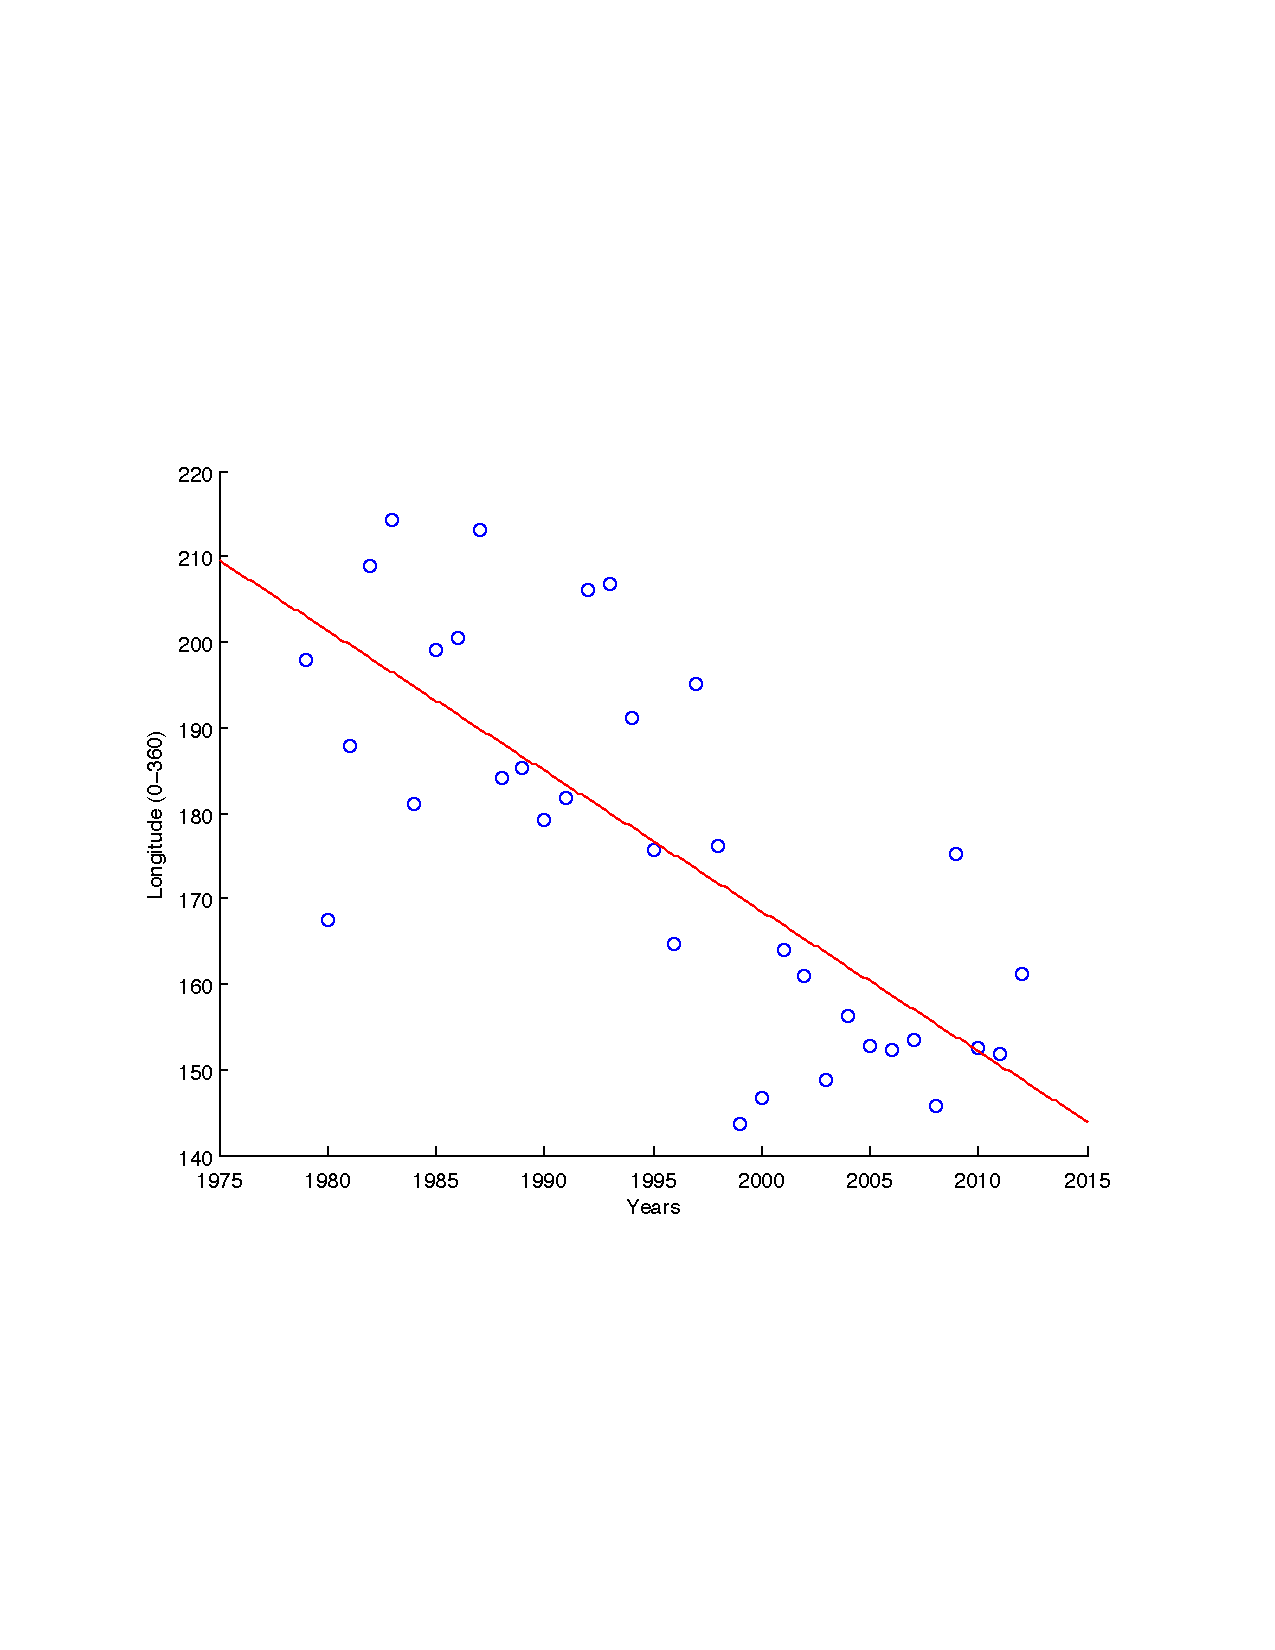
\includegraphics[height=3in]{figures/scatter.pdf}
	\caption{The annual mean longitude of the warmest SST anomaly region in the Pacific ($1979-2010$). The figure shows a clear westward shift of the warmest region in the Pacific. $R^2 = 0.54$ $p < 0.01$}
	\label{fig:figures_scatter}
\end{figure}

%This westward shift might explain traditional NINO indices' lack of accuracy. Earlier in the record, the warmest region in the Pacific might have coincided with the region's these static indices monitor, but as the warming began to shift westward the accuracy of such static indices began to deteriorate. 

\newpage